\documentclass{standalone}
\usepackage{tikz}
\begin{document}
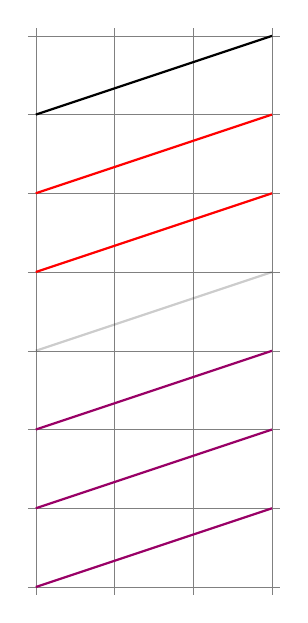
\begin{tikzpicture}[thick]
\draw[help lines] (-0.1,-0.1) grid (3.1,7.1);

\draw (0,6) -- +(3,1); % black by default
\draw[red] (0,5) -- +(3,1); % shortcut for draw=red
\draw[draw=red] (0,4) -- +(3,1);
\draw[draw opacity=0.2] (0,3) -- +(3,1);
% different ways to mix: 60% red and 40% blue
\draw[draw=red!60!blue] (0,2) -- +(3,1);
\draw[draw={rgb:red,3;blue,2}] (0,1) -- +(3,1);
\draw[draw={rgb,255:red,153;green,0;blue,102}] (0,0) -- +(3,1);

\end{tikzpicture}
\end{document}
